\section{Music to Our Ears: Standing Waves on Strings}

\makelabheader %(Space for student name, etc., defined in master.tex)

\begin{comment}
This lab was changed A LOT by Matt Trawick, 1/23/2016. Old version is saved as standing_waves_on_strings_old2015.tex.

1. Reduced the length of the background material.  Tightened up some of the exposition.  Also removed the parts that gave students the equation \lambda = 2L/n (twice!), on the grounds that students can figure it out themselves.  IMHO, the entire ``introduction'' part could still be removed and I wouldn't miss it.

2. Format changed to match the usual ``Activity 1'' etc.

3. Uncertainty is now done more consistently; students calculate uncertainty for v_A and v_B, not just v_A.

4. I removed the previous second section (`Part B') which had students change the masses to get different modes.  It's much more natural to change the frequency, and we have the equipment to do it easily.  Also, plotting T vs 1/n^2 seemed really old-timey.  And all for.... calculating the mass density, which you already knew from the scale anyway.

5.  The new section I put in instead (Activity 2) has students get different modes by changing frequency.  (This prepares them better for doing the same thing for the resonance tubes lab.)  I also have them derive, from pictures, the relationship 
f = (v/2L)n, which students always want to just memorize without thinking about it.
\end{comment}

\vspace{0.2in}

\textbf{Equipment:}
\begin{itemize} \itemsep 0pt
\item  string vibrator 
\item  sine wave generator
\item  inelastic braided string
\item  2 clamps
\item  superpulley
\item  mounting rod for the superpulley
\item  mass and hanger set
\item  precision balance
\item  tape measure or meter stick
\end{itemize}


\textbf{Introduction}

How do we make musical sounds? To make a sound, we need something that vibrates. If we want to make musical notes you usually need the vibration to
have an almost constant frequency: that means stable pitch. We also want a frequency that can be easily controlled by the player. In electronic
instruments this is done with electric circuits or with clocks and memories. In non-electronic instruments, the stable, controlled vibration is
produced by a standing wave. Here we discuss the way strings work. This is also a good introduction for studying wind instruments, because vibrating
strings are easier to visualise than the vibration of the air in wind instruments, though the math is very similar.

Waves are oscillations in an elastic medium:
\begin{itemize}
\item  your own vocal cords (the medium) vibrating as air is forced over them by your lungs; 
\item  a stretched string (the medium) on a musical instrument vibrating as it is bowed, hammered or plucked; 
\item  pressure oscillations in a column of air (the medium) in a wind instrument, organ pipe or your own oral and nasal cavities.
\end{itemize}

In each case the medium has an equilibrium state, and when displaced or otherwise perturbed from that state, experiences a force which tends to
restore it to equilibrium. For small perturbations, the restoring force is proportional to the displacement and the medium becomes a simple harmonic
oscillator.


\textbf{Background}

\textbf{Standing waves} are produced by the interference of two traveling waves, both of which have the
same wavelength $\lambda$, speed $v$, and amplitude, but travel in opposite directions through the same medium. 
One way to get standing waves is with reflections, such as when a wave traveling along a stretched string reflects off the end.  The reflected wave travels backwards, interfering with the wave traveling forwards to produce a standing wave pattern on the string.  

One characteristic of every standing wave pattern is that there are points along the medium which appear to be standing still. These points,
sometimes described as points of no displacement, are referred to as \textbf{nodes}. Points in between the nodes that undergo the \textit{maximum} displacement between
large positive and large negative valuesare called \textbf{antinodes}. When a standing wave pattern is established in a medium, the locations of nodes and antinodes remain fixed and don't move; hence the name ``standing'' waves.  A particular arrangement of nodes and antinodes is called a \textbf{mode} of vibration.

The number of nodes and antinodes in a standing wave depends the frequency of the wave as well as properties of the medium.  
If you drive a stretched string at an arbitrary frequency, you will probably not see any particular mode; many modes will be mixed together, and the overall amplitude will be small.
But, if the tension and the string's length are correctly adjusted to the frequency of the driving vibrator, one vibrational mode will occur at a much
greater amplitude than the other modes.

\begin{wrapfigure}[9]{r}{0.5\textwidth}
\vspace{-0.15in}
    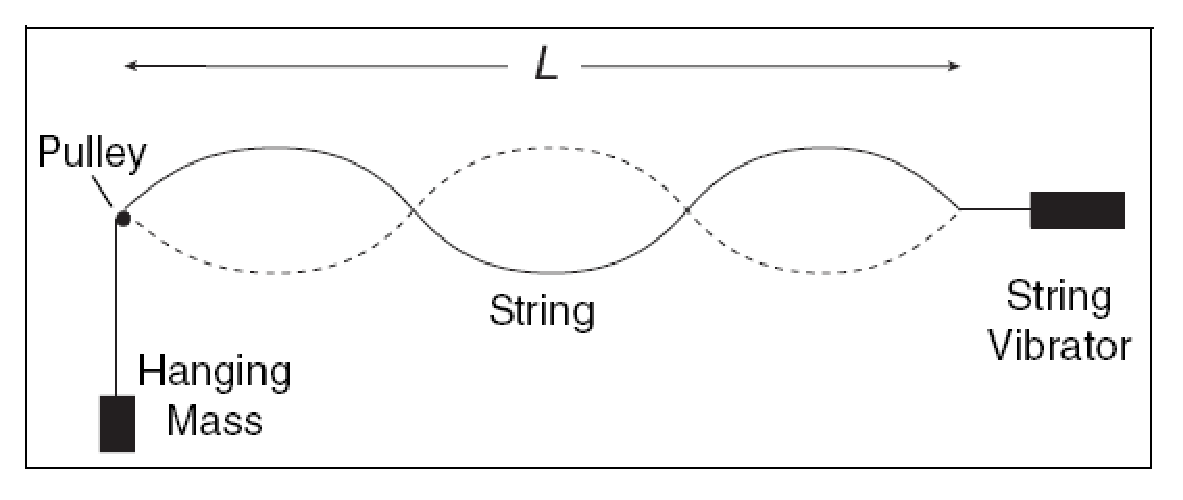
\includegraphics[width=0.5\textwidth]{standing_waves_strings/standing_waves_strings_fig2_tb.eps}
\end{wrapfigure}

\vspace{0.1in}
In this experiment, standing waves are set up in a stretched string by the vibrations of an electrically-driven string vibrator. The tension in the
string equals the weight of the masses suspended over the pulley. You can alter the tension by
changing the masses. 

%\vspace{0.3cm}
%\begin{center}
%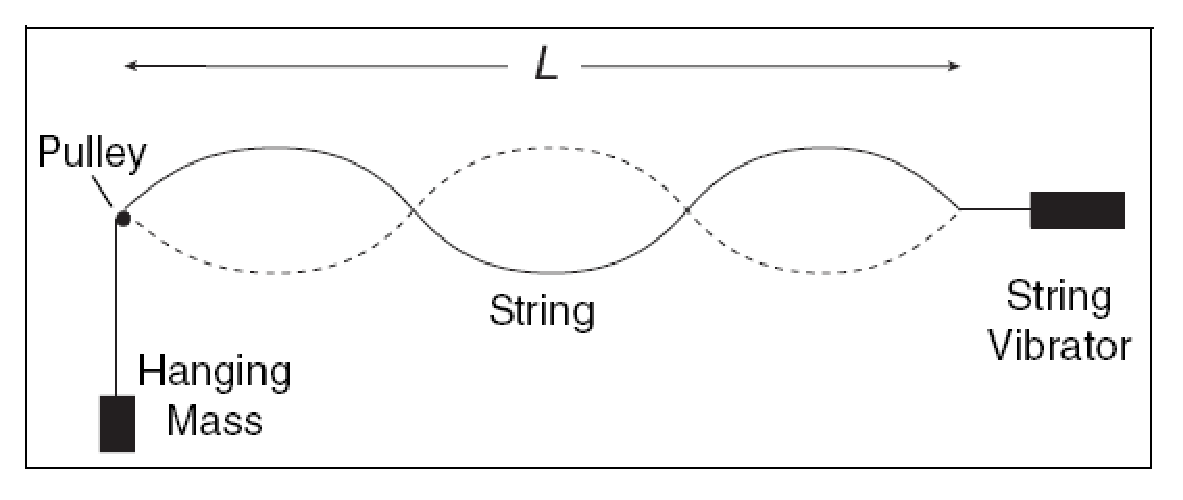
\includegraphics[width=250pt]{standing_waves_strings/standing_waves_strings_fig2_tb.eps}
%%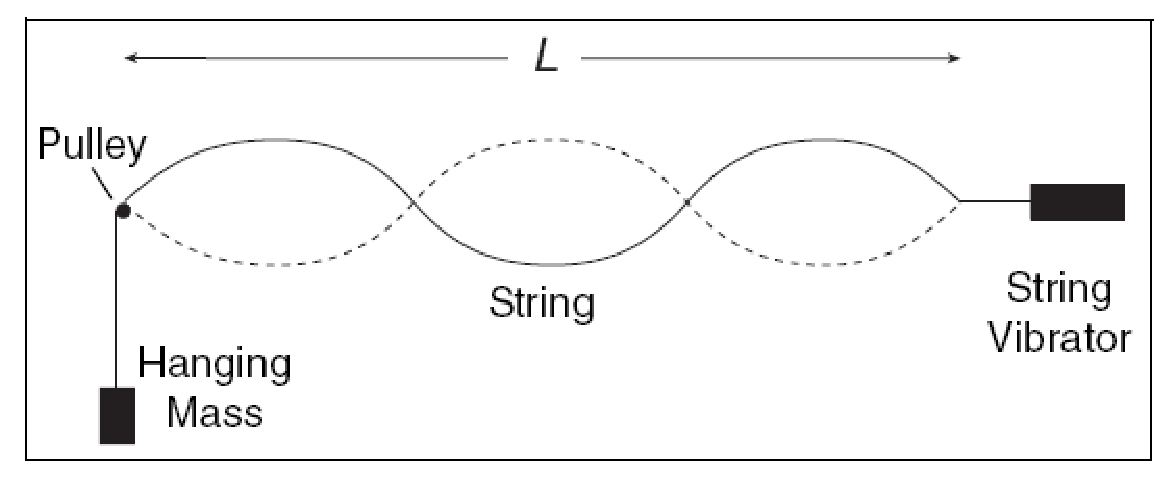
\includegraphics[width=3in]{standing_waves_strings/standing_waves_strings_figure2.eps}
%\end{center}
%\vspace{0.3cm}

The speed of a wave on the string is given by:
\begin{equation*}
v=\sqrt{\frac {T}{\mu }}
\end{equation*}
where $T$ is the tension in the string and $\mu $ is the linear density (mass/length) of the string.  The speed of any wave is also related to its wavelength and frequency by
\begin{equation*}
v=\lambda f.
\end{equation*}


\textbf{Activity 1: Varying the tension and calculating the wave speed}

(a) Measure the exact length of a piece of string several meters long. Measure the mass of the
string and calculate the linear density $\mu$ (mass/length).  (If your balance is not precise enough to measure that length of string, use a longer piece of string.)  Be sure to estimate the uncertainties in both the mass and the length, bearing in mind that the string can stretch. What is the resulting uncertainty in $\mu$?  (For help with uncertainties, refer to Appendix \ref{uncertainty}.)
\answerspace{4cm}

(b) Clamp the string vibrator and pulley about a meter apart. Attach the string to the vibrating blade, run it over the pulley, and hang about 200 g of mass from it. Cut off the excess string. Measure the distance $L$ from the knot where the string attaches to the string vibrator to the top of the pulley.
This length $L$ is NOT the total length of the string that you measured in part (a). 

Record the value here: $L$ =

\vspace{0.3cm}
\begin{center}
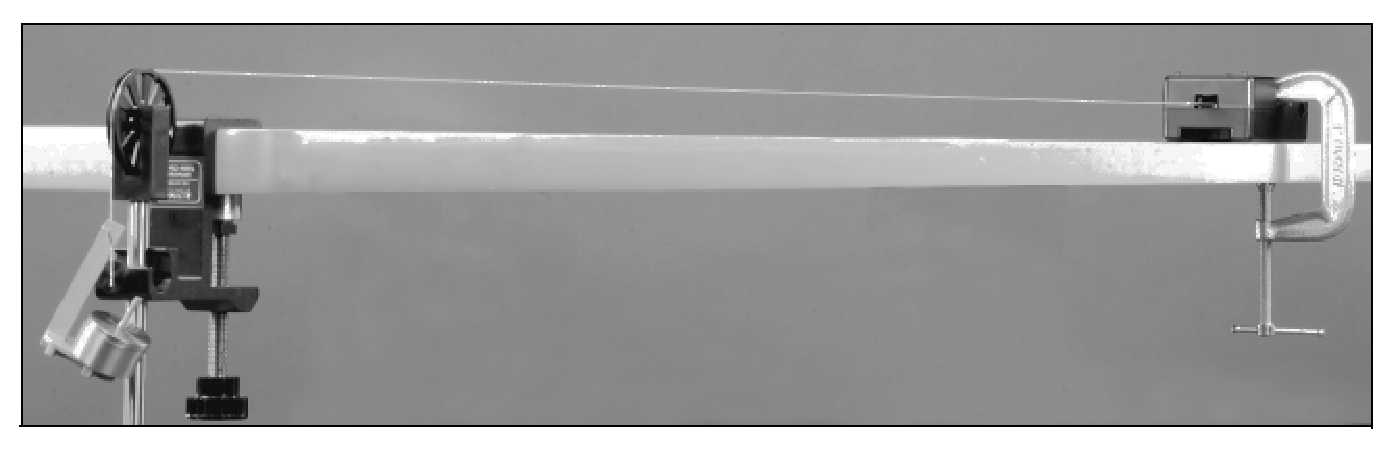
\includegraphics[width=320pt]{standing_waves_strings/standing_waves_strings_fig3_tb.eps}
\end{center}
\vspace{0.3cm}

Connect the sine wave generator to the string vibrator. (There's a tiny switch in the back of the generator to turn it on.)  Adjust the frequency to 60.0 Hz, and adjust the amplitude to a moderately high value.

Change the tension by adding to or subtracting from the hanging mass so that the string vibrates in 2 segments. Adjust the tension to achieve a ``clean'' node at the center. Also check the end of the vibrating blade; the point where the string attaches should be a node. It is more important to have a good node at the blade than it is to have the largest amplitude possible. However, it is desirable to have the largest amplitude possible while keeping a good node.

(c) Record the hanging mass, $m$. How much uncertainty is there in your value? By how much can you change the hanging mass before you see an effect? Record the uncertainty.
\answerspace{1cm}

(d) Calculate the tension $T$ (including the uncertainty) in the string.
\answerspace{2cm}

\pagebreak[3]

(e) Calculate the speed $v_A$ of the wave from your observed values of tension
$T$ and linear density $\mu$. Record your calculated value with the uncertainty and the correct number of significant
figures.
\answerspace{4cm}

(f) Calculate the speed $v_B$ from the wavelength ($\lambda $) and frequency ($f$).  What are your uncertainties in $\lambda$ and $f$?  What is your uncertainty in $v_B?$
\answerspace{4cm}

(g) Compare the two values of speed, $v_A$ and $v_B$.  Are the two consistent, to within the uncertainties you calculated?  That is, do their ranges overlap?  (If not, you have some explaining to do....) 
\answerspace{3cm}

\pagebreak[2]
\textbf{Activity 2: Vibrational modes at different frequencies}

\textit{For this part, keep the same string length as in Activity 1, and keep about 200 grams on the end of the string.}

(a) In Activity 1, the standing wave on the string had one node in the middle, dividing the string into $n=2$ vibrating segments.  This means that the standing wave had $n=2$ antinodes.  Change the frequency to find both higher and lower values of $f$ that produce standing waves with different numbers of antinodes.  Record your results in the table below.
\begin{center} 
\begin{tabular}{|c|c|} 
\hline $\mathbf{n}$ & \boldmath$f$ \textbf{(Hz)} \\ 
\hline 1 &  \\ 
\hline 2 &  \\ 
\hline 3 &  \\ 
\hline 4 &  \\ 
\hline 5 &  \\ 
\hline 6 &  \\ 
\hline 7 &  \\ 
\hline 
\end{tabular} 
\end{center}

(\textit{You may need to adjust the amplitude knob to keep the standing wave a reasonable size.  Also, don't worry if the last few modes are too hard to see.  Finally, there's a weird resonance within the string vibrator itself that makes it wonky around 150 Hz; just ignore that and skip past it if necessary.})

\pagebreak[3]

(b) On the lines below, draw pictures of the first three standing wave modes you found.  For each drawing, write the relationship between the half wavelength $\frac{1}{2}\lambda$ and the string length $L$.

\begin{center}
$n=1$: 
\raisebox{-0.15in}{\rule{3pt}{0.4in}}\raisebox{.05in}{\rule{2.5in}{0.1pt}}\raisebox{-0.15in}{\rule{3pt}{0.4in}}
\hspace{0.3in}$\frac{1}{2}\lambda=$

$n=2$:
\raisebox{-0.15in}{\rule{3pt}{0.4in}}\raisebox{.05in}{\rule{2.5in}{0.1pt}}\raisebox{-0.15in}{\rule{3pt}{0.4in}}
\hspace{0.3in}$\frac{1}{2}\lambda=$

$n=3$:
\raisebox{-0.15in}{\rule{3pt}{0.4in}}\raisebox{.05in}{\rule{2.5in}{0.1pt}}\raisebox{-0.15in}{\rule{3pt}{0.4in}}
\hspace{0.3in}$\frac{1}{2}\lambda=$
\end{center}
%axes

(c) From your three pictures above, write a general equation relating $\lambda$ and $L$ for each possible value of $n$.
\answerspace{2cm}

(d) Using the relationship between $\lambda$, $f$, and $v$, rewrite your equation in (c) to express the frequency $f$ for each value of $n$, in terms of $n$, $v$, and $L$.
\answerspace{2cm}

(e) If you were to make a graph of $f$ \textit{vs.} $n$, what would be the slope of that graph, in terms of $v$ and $L$?
\answerspace{2cm}

\pagebreak[3]
(f) Plot a graph of your data for $f$ vs $n$ from part (a) using Excel. Use the LINEST function to determine the slope of the graph and its uncertainty. From these values, calculate the velocity of the wave, and its uncertainty, and record them here. (See Appendix \ref{excel} for help using Excel's LINEST function.  Also, do you want LINEST to estimate the $y$-intercept, or force it to zero?)
\answerspace{4cm}

(g) Is your result for (f) consistent with the values $v_A$ and $v_B$ you calculated in Activity 1?  Does the uncertainty in the slope given by LINEST capture \textit{all} sources of uncertainty in your measurement?
\answerspace{4cm}


\textbf{Further Investigation}

If a strobe is available, observe the standing wave on a string with the 
strobe light. Draw a diagram explaining the motion of the string.




